\section*{1.1 - Requisiti (...)}
Si vuole realizzare un sistema software che offra un servizio di sharing musicale, unito alle funzionalità tipiche di un social network. Alla registrazione, l'utente dovrà inserire una lista di generi musicali preferiti. L'algoritmo proporrà quindi all'utente i brani più popolari basati sulle sue preferenze e gli permetterà di esplorare le sue affinità musicali. Gli attori in gioco sono i seguenti: \par
\begin{itemize}
    \item  utenti che vogliono ascoltare musica, conoscere e condividere le proprie attività musicali con gli amici;
    \item  artisti indipendenti e non per pubblicare e gestire la propria musica.
\end{itemize}
\par
L'utente, per poter usufruire dei servizi forniti, deve registrarsi e creare un proprio profilo personale. Una volta iscritto, verrà indirizzato alla homepage che mostra i brani più popolari dei generi preferiti dall'utente, la possibilità di cercare un brano specifico e la sezione di impostazioni personali e social. Quando viene selezionato il brano da scaricare, vengono fornite tutte le informazioni relative (titolo, artista, album, anno di uscita, genere di appartenenza, numero di ascolti, durata del brano, casa discografica).
\par 
Il software offre anche la possibilità di mettere “like" ai brani e di creare playlist personalizzate. Nella propria libreria saranno quindi presenti le playlist dell'utente e la playlist dei brani preferiti. L'interfaccia social permette invece di aggiungere gli amici e di chattare con essi.
\par 
La funzionalità principale offerta dal servizio è l'algoritmo “Discover", che consente di trovare i brani più apprezzati dalle persone che ascoltano gli stessi generi musicali dell'utente così da permettergli di scoprire sempre nuove canzoni.
\par 
L'artista, a differenza dell'utente ascoltatore, può caricare brani singoli e album inserendo i dati relativi alla propria produzione artistica. 
\par
L'utente, per poter usufruire dei servizi forniti, deve registrarsi e creare un proprio profilo personale. Una volta iscritto, verrà indirizzato alla homepage che mostra i brani più popolari dei generi preferiti dall'utente, la possibilità di cercare un brano specifico e la sezione di impostazioni personali e social. Quando viene selezionato il brano da scaricare, vengono fornite tutte le informazioni relative (titolo, artista, album, anno di uscita, genere di appartenenza, numero di ascolti, durata del brano, casa discografica).
\par
Il software offre anche la possibilità di mettere “like" ai brani e di creare playlist personalizzate. Nella propria libreria saranno quindi presenti le playlist dell'utente e la playlist dei brani preferiti. L'interfaccia social permette invece di aggiungere gli amici e di chattare con essi.
\par 
La funzionalità principale offerta dal servizio è l'algoritmo “Discover", che consente di trovare i brani più apprezzati dalle persone che ascoltano gli stessi generi musicali dell'utente così da permettergli di scoprire sempre nuove canzoni.
\par
L'artista, a differenza dell'utente ascoltatore, può caricare brani singoli e album inserendo i dati relativi alla propria produzione artistica. 

\vspace*{3em}

\section*{1.2 - Studio di fattibilità (...)}
Procedendo con una valutazione dei costi e dei benefici della possibile realizzazione del presente sistema, è possibile concludere che i costi principali sono relativi alla funzionalità di Discover e brani consigliati. Per realizzare questa funzionalità è necessaria l’implementazione di un algoritmo che vada a studiare i gusti e le preferenze di ogni singolo utente e, dopo la preliminare fase di raccolta dati, proporrà all’utente una serie di brani in linea con le sue preferenze. par
Per quanto riguarda invece la fattibilità in termini di tecnologie e strumenti per la realizzazione del sistema (...)

\section*{1.3 - Casi d'uso}
Di seguito vengono riportati i casi d’uso raggruppati in base all’attore coinvolto. Come anticipato gli attori in gioco sono i seguenti:
\begin{itemize}
    \item Utente ascoltatore;
    \item Artista (indipendente/non);
\end{itemize}

\subsection*{1.3.1 - Casi d'uso utente}
\begin{itemize}
    \item \textbf{UC1}: Sign in \par
        L’utente può registrarsi inserendo le sue informazioni personali.
    \item \textbf{UC2}: Log in \par 
        L’utente può accedere al proprio profilo personale inserendo nome utente e password.
    \item \textbf{UC3}: Log out \par 
        L’utente può disconnettere il proprio profilo personale dal sistema.
    \item \textbf{UC4}: Consulta home-page \par 
        L’utente può navigare nelle varie sezioni della home page.
    \item \textbf{UC5}: Cerca brano \par 
        L’utente può digitare nella barra di ricerca per cercare un brano dal titolo.
    \item \textbf{UC6}: Scarica brano \par
        L’utente può scaricare il brano.
    \item \textbf{UC7}: Like al brano \par 
         L’utente può esprimere il proprio interesse per un brano mettendo like.
    \item \textbf{UC8}: Aggiungi brano a playlist \par 
        L’utente può aggiungere alla lista di brani della playlist un brano selezionato.
    \item \textbf{UC9}: Cerca Utente \par 
        L’utente può cercare un utente per nome dalla barra di ricerca apposita (cerca album/artista).
    \item \textbf{UC10}: Aggiungi Utente \par 
        L’utente può aggiungere alla propria lista amici un utente selezionato.
    \item \textbf{UC11}: Visualizza informazioni profilo \par 
        L’utente può consultare le proprie informazioni personali inserite in fase di registrazione. 
    \item \textbf{UC12}: Modifica profilo \par 
        L’utente può modificare le proprie informazioni personali inserite in fase di registrazione.
    \item \textbf{UC13}: Elimina profilo \par 
        L’utente può eliminare il proprio profilo dal sistema. 
    \item \textbf{UC14}: Visualizza playlist \par 
        L’utente può consultare tutte le proprie playlist.
    \item \textbf{UC15}: Crea nuova playlist \par 
        L’utente può creare una nuova playlist nella quale aggiungere brani.
    \item \textbf{UC16}: Elimina playlist \par 
        L’utente può eliminare una delle proprie playlist.
    \item \textbf{UC17}: Modifica playlist \par 
        L’utente può modificare una delle proprie playlist, per esempio modificando il nome o rimuovendo brani.
    \item \textbf{UC18}: “Discover” e classifiche \par 
        L’utente può consultare classifiche e brani scelti per lui dal sistema.
    
\end{itemize}

\newpage

\subsection*{1.3.2 - Casi d'uso artista}
\begin{itemize}
    \item \textbf{UC19}: Crea pagina artista \par 
        L’artista per poter pubblicare musica deve creare una pagina artista inserendo le proprie informazioni personali.
    \item  \textbf{UC20}: Visualizza pagina artista \par
        L’artista può consultare la propria pagina artista, dove vengono visualizzati i propri brani/album pubblicati.
    \item  \textbf{UC21}: Aggiungi brano \par 
        L’artista può pubblicare un nuovo brano inserendo le informazioni relative.
    \item  \textbf{UC22}: Aggiungi album \par
        L’artista può pubblicare un nuovo album contente i brani scelti.
    \item  \textbf{UC23}: Personalizza pagina artista \par 
        L’artista può decidere quali brani e album mettere in evidenza nella propria pagina artista. 
    \item  \textbf{UC24}: Consulta anagrafica \par 
        L’artista può consultare l’anagrafica relativa agli ascolti e ai like dei brani e album pubblicati. 
    
\end{itemize}



\subsection*{1.3.3 - Dettaglio casi d'uso (...)}
\par 

\newpage
\subsection*{1.3.4 - Diagramma dei casi d'uso}
In figura è stato riportato il diagramma dei casi d’uso, dove sono stati inseriti quelli già precedentemente descritti mettendoli in correlazione con il corrispettivo attore.
    \begin{figure}[H]
        \centering
        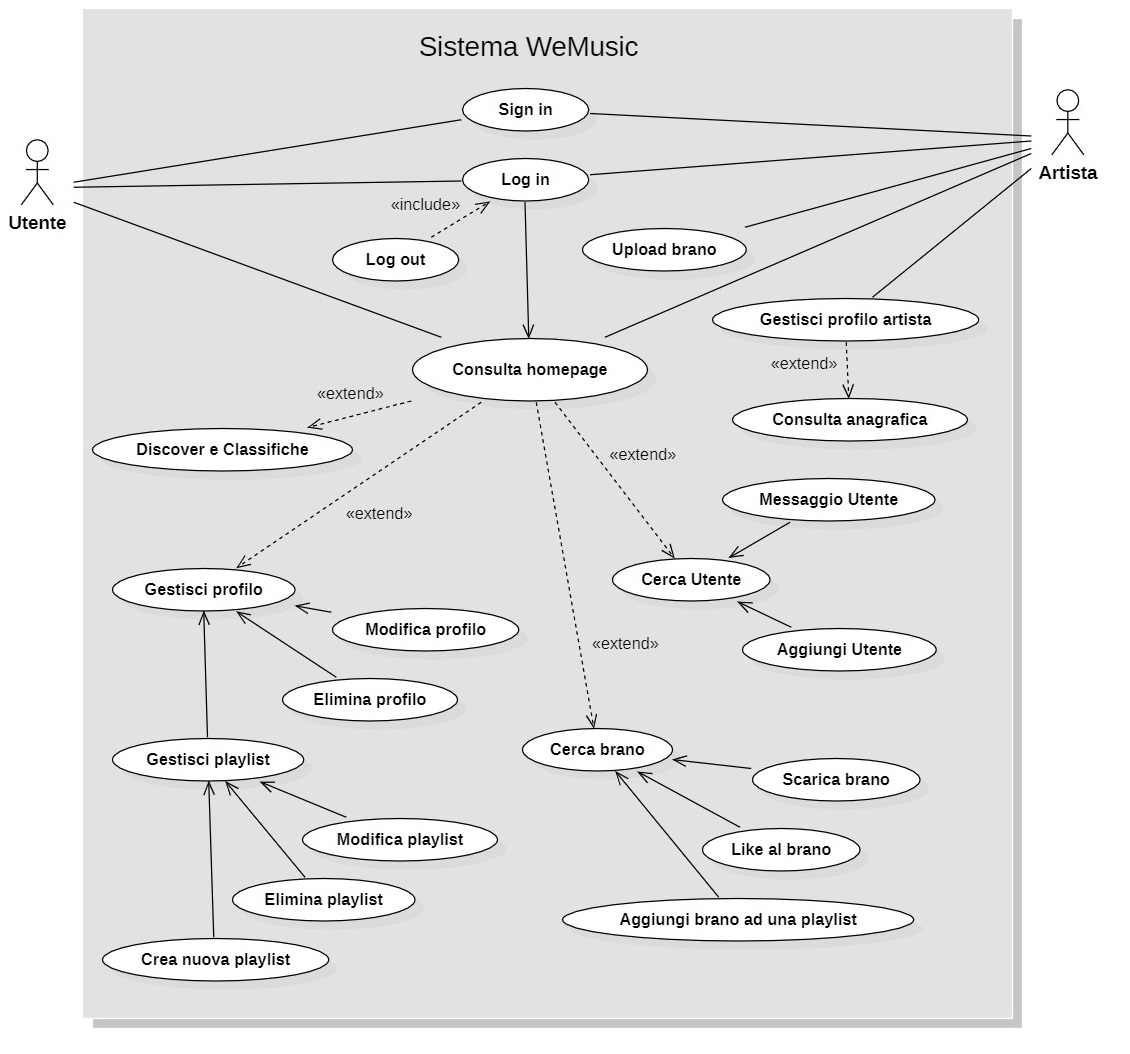
\includegraphics[scale=0.50]{UseCaseDiagramver1.jpg}
        \caption[]{UML use cases diagram}
    \end{figure}

\newpage

\section*{1.4 - Architettura del sistema(...)} 






\subsection*{1.4.1 - Deployment diagram - Informal}






\subsection*{1.4.2 - Deployment diagram - UML}






\newpage

\section*{1.5 - Toolchain e tecnologie utilizzate (...)}